%% Template for SDP report, adapted from mlp_cw2_template, 2018. 

%% Based on  LaTeX template for ICML 2017 - example_paper.tex at 
%%  https://2017.icml.cc/Conferences/2017/StyleAuthorInstructions

\documentclass{article}
\usepackage{pifont}
\usepackage[T1]{fontenc}
\usepackage{amssymb,amsmath}
\usepackage{txfonts}
\usepackage{microtype}
\usepackage{xspace}
\xspaceaddexceptions{\%}
\usepackage{subcaption}
% Lists with less spacing between items
\usepackage{paralist}
\usepackage{tabularx}
\usepackage[normalem]{ulem}
% For figures
\usepackage{graphicx}
\usepackage{subfig} 

% For citations
\usepackage{natbib}

% For algorithms
\usepackage{algorithm}
\usepackage{algorithmic}

% the hyperref package is used to produce hyperlinks in the
% resulting PDF.  If this breaks your system, please commend out the
% following usepackage line and replace \usepackage{mlp2017} with
% \usepackage[nohyperref]{mlp2017} below.
\usepackage{hyperref}
\usepackage{url}
\urlstyle{same}

% Packages hyperref and algorithmic misbehave sometimes.  We can fix
% this with the following command.
\newcommand{\theHalgorithm}{\arabic{algorithm}}


% Set up MLP coursework style (based on ICML style)
\usepackage{mlp2018}
\mlptitlerunning{SDP Demo \demoNumber  Group (\groupNumber)}
\bibliographystyle{icml2017}


\DeclareMathOperator{\softmax}{softmax}
\DeclareMathOperator{\sigmoid}{sigmoid}
\DeclareMathOperator{\sgn}{sgn}
\DeclareMathOperator{\relu}{relu}
\DeclareMathOperator{\lrelu}{lrelu}
\DeclareMathOperator{\elu}{elu}
\DeclareMathOperator{\selu}{selu}
\DeclareMathOperator{\maxout}{maxout}






\usepackage{titlesec}


\newcommand{\cmark}{\ding{51}}%
\newcommand{\xmark}{\ding{55}}%

\setlength{\itemsep}{0mm}%
\setlength{\parskip}{0mm}
%% You probably do not need to change anything above this comment

%% REPLACE the details in the following commands with your details
\setGroupNumber{4}
\setGroupName{Sprout.ed}
\setProductName{Sprout.ed}
\setDemoNumber{3}
\setLogoFileName{figs/sprouted_logo.png}

\begin{document} 

\makeSDPTitle{Demo}

% Previous MLP Style Title Layout working. 
% \twocolumn[
    % \mlptitle{\productName: SDP Demo \demoNumber}
    % \centerline{Group \groupNumber: \groupName}
% ]

\begin{abstract}
Sprout.ed is a 3-axis automated planting and watering system designed for office space well being, with a web app allowing for an overview and management of the plantbed. 

Sprout.ed has bloomed since the last demo, and now implements a custom split drill head which can dig and cover seeds into the soil, allowing for automated planting when combined with the addition of the air pump to pick up, hold and drop seeds. The functionality of the webcam was extended with computer vision, allowing the system to avoid plants when testing moisture levels and adjusting water needs once the plant becomes a seedling. The web app has taken great strides, displaying logs of actions carried out by the system and now boasts an interface to visualise the current plantbed where plants can be added to spaces suitable for each plant type. Throughout all sub-teams, comprehensive quantitative analysis was carried out and used to adjust designs and processes.
\end{abstract} 

\section{Project plan update} 

\subsection{Milestone 3 goal updates}
We were organised into three sub-teams again working towards this milestone.
\subsubsection{\textbf{Mechanical Team - Anukrat, Rokas, Yichao}}

\vspace{1mm}
\begin{itemize}
    \setlength\itemsep{0.01em}
    \setlength\parskip{0pt}
    \item (Achieved) Digging/drilling utensil
    \item (Partly achieved, see Section \ref{sec:covid}) Watering system
    \item (Achieved) Seed deployment system
\end{itemize}

The subteam's main objective was designing a compact 5-purpose robotic arm solution. It will be able to dig holes in the soil, transport seeds from containers to the holes, cover the seeds up with soil, water them as they grow and take moisture readings. To achieve these goals, Rokas and Yichao designed and prototyped numerous models for the solution. They also jointly designed the modular (by LEGO connectors) seed containers and seed chamber resting at the end of the vacuum tube. Yichao proceeded to CAD model and 3-D print these parts. In addition, Rokas added a motor controller board connected to Raspberry Pi to the system. Anukrat joined the electrical team to help set up the new motors and make spreadsheets for quantitative analysis. We also redesigned the 3-D printed LEGO adaptor (as introduced in Demo 1) for stronger stability.

\subsubsection{\textbf{Electrical Team - Alan, Shreyas, Serena, Terry}}
\vspace{3mm}

\vspace{1mm}
\begin{itemize}
    \setlength\itemsep{0.01em}
    \setlength\parskip{0pt}
    %\vspace{-3mm}
    \item (Achieved) Digging/drilling related movements
    \item (Partly achieved - see Section \ref{sec:covid}) Automated  watering
    \item (Achieved - Part of Milestone 4) Air Pump picking and dropping seeds
    %\vspace{-5mm}
\end{itemize}
Alan worked with Rokas to achieve digging/drilling related movements and also completed part of the next milestone: using the air pump to pick seeds and drop them. Anukrat, Shreyas, Balraj and Serena worked on the quantitative analysis (QA), testing the air pump with different sizes of seeds and testing the drill movements with various soils and moisture levels. Terry worked on an extension - using computer vision, allowing us to use the webcam to adjust arm movement to avoid plants. The subteam then started working on joining the computer vision and sensor readings to build the logic that controls Automated Watering (see Figure \ref{fig:pseudocode} for pseudo-code).


\subsubsection{\textbf{Web App Team -  Balraj, Dima, Sonia}}
\vspace{1mm}
\begin{itemize}
    \setlength\itemsep{0.01em}
    \setlength\parskip{0pt}
    %\vspace{3mm}
    \item (Achieved) Action history and error log
    \item (Achieved) Implement plant dashboard
    \item (Achieved) Implement watering controls
    %\vspace{-4mm}
\end{itemize}

Dima implemented the plant dashboard using React, creating both a user and admin mode, and giving the admin mode the add/remove plant feature with watering controls and researched for the watering logic. Sonia implemented the action log using Datatables and carried out the quantitative analysis for the web app. Balraj worked on an admin log in for the web app and worked with the Electrical team to perform quantitative analysis of the robot.

\subsection{Milestone 4 Goals}
The following would be the goals for Milestone 4, if work could continue for Demo 4.
\vspace{1mm}

Mechanical Team:
\vspace{-3mm}

\begin{itemize}
    \setlength\itemsep{0.01em}
    \setlength\parskip{0pt}
    \item Watering system - represent watering e.g.  using light
    \item Branded covers for untidy components of robot
\end{itemize}
%\vspace{-2mm}
Electrical Team:
\vspace{-3mm}
\begin{itemize}
    \setlength\itemsep{0.01em}
    \setlength\parskip{0pt}
    \item Automated seed planting - Picking the desired seed and dropping it in the desired location. 
    \item Integration of webcam and sensor readings with the seeding and watering \item Final testing of every functionality
    %\vspace{-3mm}
\end{itemize}
Web App Team:
\vspace{-3mm}

%\vspace{1mm}
\begin{itemize}
    \setlength\itemsep{0.01em}
    \setlength\parskip{0pt}
    \item Fix issues identified by QA and evaluation
    \item Gather final info for plant DB - e.g. types of suitable plants, their growth radius and growth rate data.
    \item All system functionality can be carried out directly through webapp.
    %\vspace{-3mm}
\end{itemize}


\section{Technical details}

\subsection{Mechanical}

\subsubsection{Watering System}
The watering system was planned to involve an LED strip to visually represent the flow of water. However, these proved prohibitively expensive and an alternative was considered. In keeping with the idea of representing water with light, we opted to use an optics fibre. However, after removing the outer coating and testing, it proved to not have the behaviour we wanted, namely lighting up the entirety of the fibre as light travels through it. Alternatives for water representation are still being considered.

\subsubsection{Digging/drilling utensil}
\begin{figure}[h]
\begin{center}

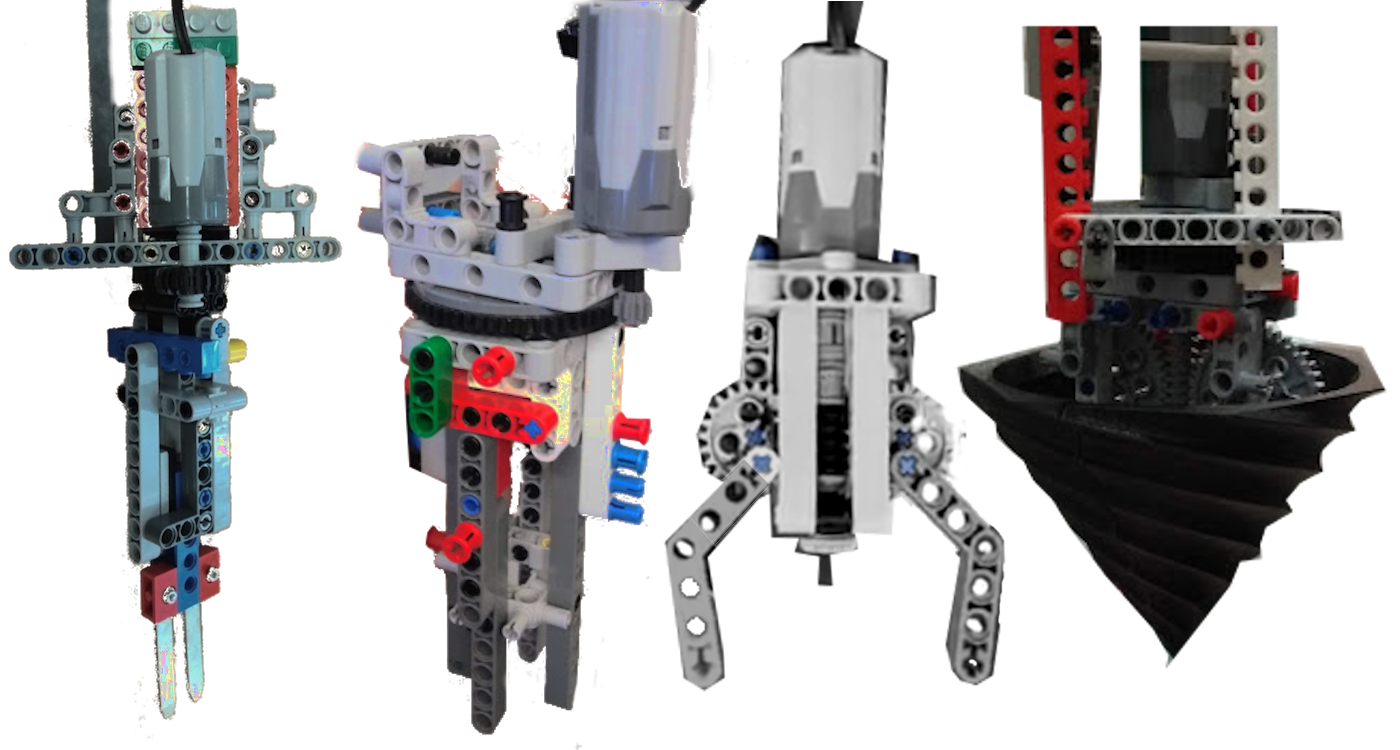
\includegraphics[width=0.8\linewidth]{figs-demo3/drill-iters.png}

\caption{iterations of the digging utensil, first iteration being on the left, progressing to the right, and finishing with the current iteration. }
\label{fig:drills}
\end{center}
\vskip -4mm
\end{figure} 

The drilling utensil proved to be the most challenging part of the hardware. Both design and implementation-wise, due to the need of having a lot of functionality within a small space. We went through numerous iterations of this piece, most noteworthy ones can be seen in Figure \ref{fig:drills}. The final iteration involves two custom printed drill halves which can rotate and open/close in a claw-like motion. Enclosed by the drill there is the vacuum nozzle (also printed) and the moisture sensor. 



This design achieves goals we set out for the planting process:
\begin{itemize}
\vspace{-1mm}
\item Piercing/softening of soil with the rotational motion of the drill
\item Planting the seed by dispensing it into the hole and burying it by the closing motion of the claw. The method of planting is depicted in Figure \ref{fig:method}
\item Securing the moisture sensor during digging to avoid damaging it.
\end{itemize}
\vspace{-5mm}

\begin{figure}[h]
\begin{center}

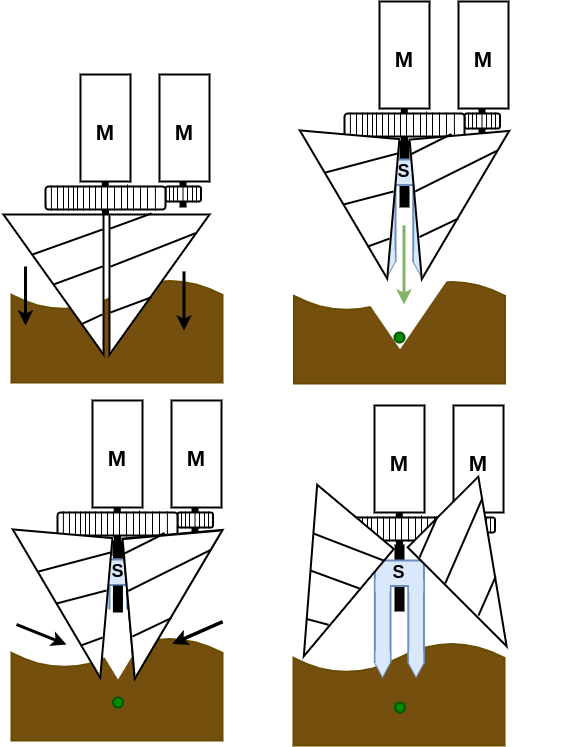
\includegraphics[width=0.6\linewidth]{figs-demo3/method.png}

\caption{Images depicting the process of planting and covering the seed, as well as taking a moisture reading. \textbf{M} marks motors. \textbf{S} marks the sensor.  }
\label{fig:method}
\end{center}
\vskip -4mm
\end{figure} 

\subsubsection{Seed Deployment}
For picking up and dropping seeds, an air pump was used. The air pump was positioned on the gantry, connecting to a thinner tube in an air-tight fashion to allow us to fit the seed dispenser inside the drill, and 3D printing a custom part which secures the tube in place and contains a filter to catch seeds. This design ensures seeds do not get stuck inside the tubing and simplifies circuitry (requiring only one direction of air flow from the pump). 

\subsection{Electrical}

\subsubsection{Computer Vision}

We initially set up a camera to allow users to simply view plants on the plant bed but alongside assessor feedback we found ways to increase functionality of the robot. The camera is now positioned on the head pointing straight down and is used to detect whether a position has a plant or not  which helps us know whether or not the arm can move down to pierce the soil or needs to offset the soil moisture measurement. Additionally, by detecting when a plant has sprouted we adjust the water it requires, as seedlings require more.

We considered building a 2D Convolutional Neural Network with TensorFlow \cite{TF} to implement image classification at first. However, training the CNN would need a huge training dataset and the accuracy would vary a lot due to different plant species. So we switched to use Pillow \cite{Pillow} and OpenCV \cite{opencv_library} modules to implement the function in following steps:

\begin{enumerate}
    \vspace{-2mm}
    \item Process the picture from the webcam and extract target color green (representing plants) by setting RGB boundaries to find any shades of green.
    \item Convert the extracted picture to binary(convert target color to white, otherwise black)
    \item Cut the picture into 9 identical squares and calculate ratio of black pixels among the region to get approximate distance.
    \item Pick out the nearest square that doesn't have a plant and instruct the robot to move to that point.
    \vspace{-1mm}
\end{enumerate}

\subsubsection{Digging/Drilling + Seed Picking and Dropping}

To achieve the digging movements we first had to set up a separate circuit to source power from an external battery pack which was done with the help of the SDP wiki. Once the motor movements were set up, we went through several iterations of sequencing the drill movements. We initially implemented a drill that pierces the soil, opens the claws, drops the seed and then goes back up. While testing this, we realized that the resistance of the soil was too high and this made opening the claws too difficult. We had also missed out the covering of the hole after the process.

After planning with the mechanical team we came up with our current implementation which can be seen in Figure \ref{fig:method}.

\begin{enumerate}
    \vspace{-3mm}
    \item The drill pierces the soil and then the arm goes up
    \item The claws open and drop the seed into the hole
    \item The arm goes to soil level and the claws close while covering the hole with soil.
    \vspace{-3mm}
\end{enumerate}

After finalising implementation details, we successfully set up the air pump and next step is to write the code to pickup seeds from a container and drop it in the desired spot, as part of the drill sequence.


\subsubsection{Automated Watering Logic}

Figure \ref{fig:pseudocode} shows the psuedocode produced to control the automated watering. This is yet to be implemented due to the situation with Covid-19 (see Section \ref{sec:covid}).

\begin{figure}[h]
\begin{center}

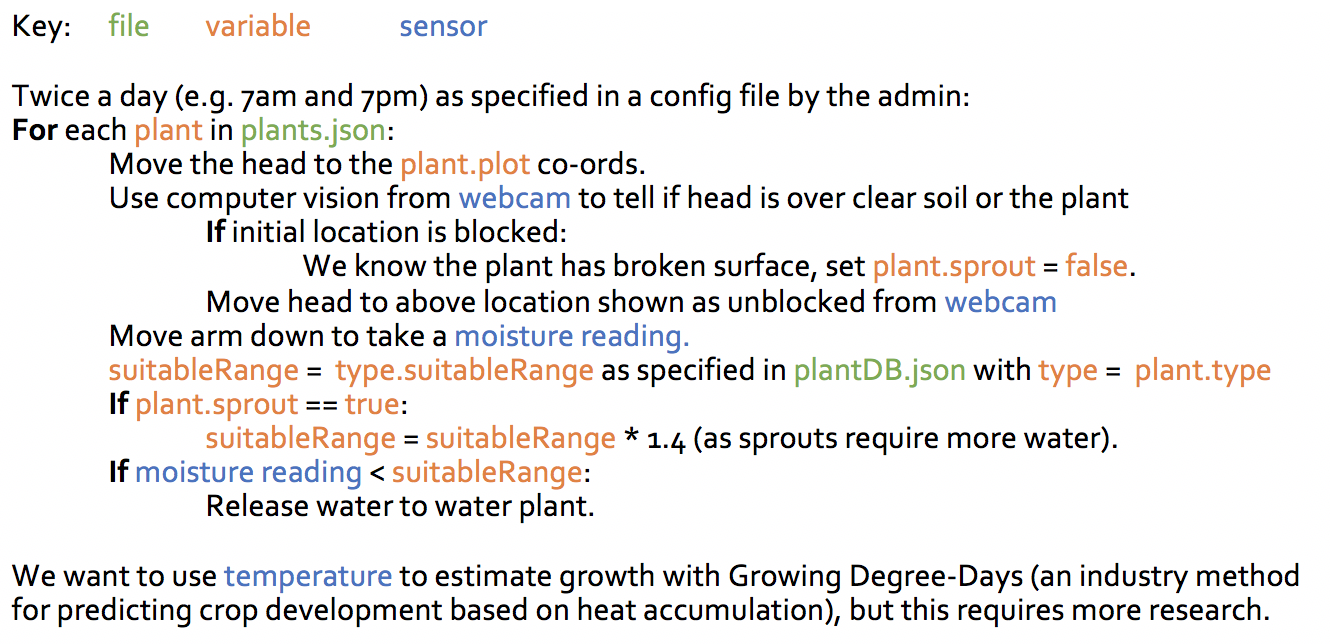
\includegraphics[width=1.075\linewidth]{figs-demo3/pseudoCode.png}

\caption{Pseudocode of the current watering logic system. \\ Growing Degree-Days reference: \cite{MSU}}
\label{fig:pseudocode}
\end{center}
\vskip -4mm
\end{figure} 

The moisture sensor we opted to use is the Grove moisture sensor, which determines moisture by passing a current through the soil and determining the resistance \cite{GMS}. For this method, re-calibration only becomes necessary when extreme temperature changes occur or with different types of soil \cite{MDPI}, by monitoring temperature and calibrating when sprout.ed is first set up, we can control for both of these factors. 

\subsection{Web App}

\subsubsection{Action Log}

To display the action log, we have used \href{https://datatables.net/}{DataTables}, a jQuery plug-in recommended to us by a previous SDP student who had to display data in a similar setting. Using this plug-in made it quick to add advanced features to our HTML table, such as multiple pages and a search feature, rather than building in these features ourselves from scratch. We use an Ajax request to get the data from a JSON file to display in the table. Actions are logged by being added to this JSON file. We realise however that this action log records actions that are requested on the web app, and does not necessarily confirm that the corresponding action of the robot has taken place in the physical world - solutions to log the confirmation of robot actions are being explored.

\subsubsection{Plant Dashboard}

The plant dashboard has now been implemented, using React. The plant bed is split up into plots with data for the plants and information on their types being loaded from JSON files. The dashboard has several modes: on the user mode, users can see where plants are located in the plant bed and click on them for more information. In the admin mode, it is also possible to add a new plant to the bed, and to remove existing plants. When the web app and the back-end system are linked up, adding the plant in the web app will cause the seed to be planted in the real life plant bed. From the admin mode there is also the option to select plants to water as a manual override to the automated watering.

The add plant feature uses an  interface alike to drag and drop to choose the plot in which to sow the seed (see Figure \ref{fig:add_plant}). Each plant type has a set radius (loaded from our plant database JSON) which limits how close it can be sowed to other plants. After selecting a plant type, when the cursor hovers over a suitable location, all the plots within the radius turn green to indicate the suitability of the location. If the cursor is over an unsuitable location, the plots within the radius turn grey to indicate this, and the plot reserved by other plants turn red to indicate where the problem is. These colour changes give instant guidance to the user on their actions, improving usability.

We decided to use emojis as an abstract representation of the plants on the dashboard. We considered displaying a photo of the plant, but decided that it worked better to only show the photo when the user requests more information about a plant, instead of photographs being integrated into the virtual plant bed itself.

\begin{figure}[h]
\begin{center}

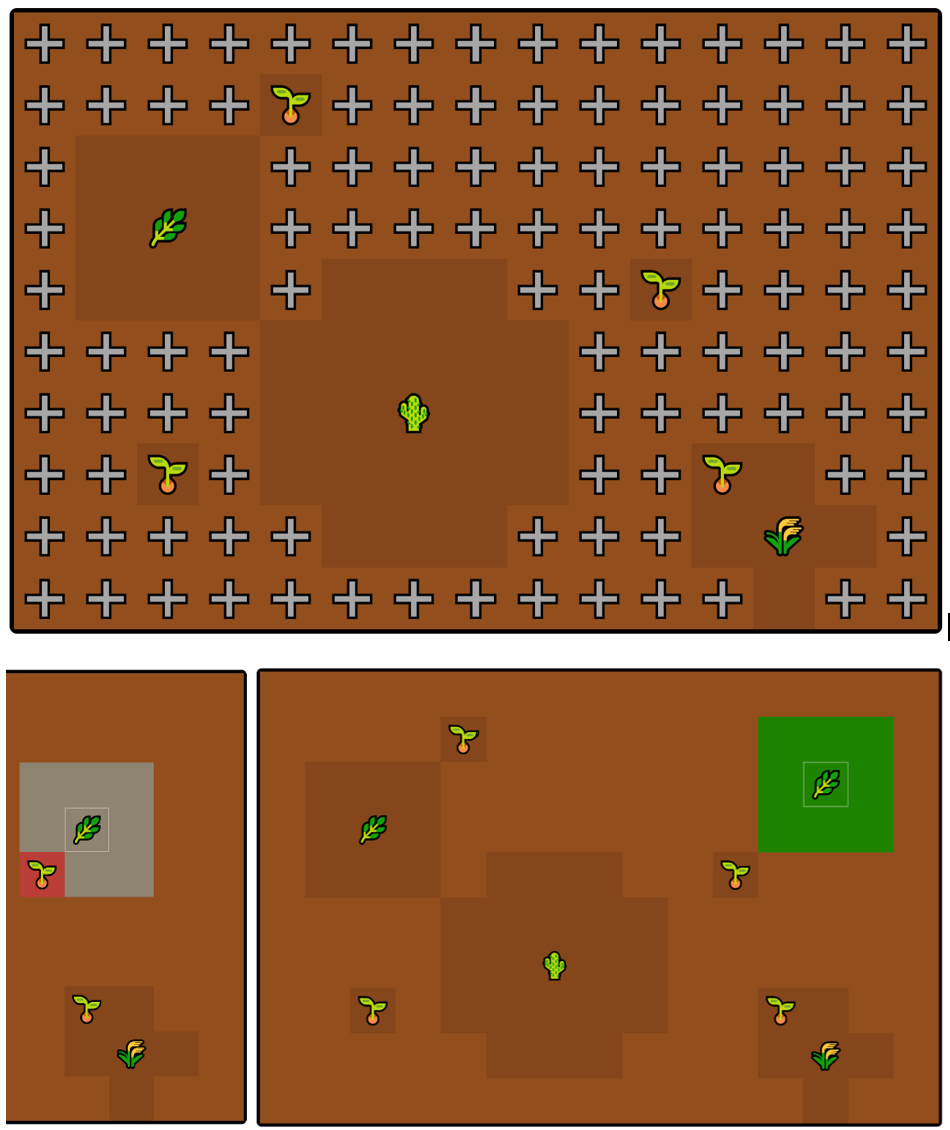
\includegraphics[width=0.8\linewidth]{figs-demo3/add_plant.png}

\caption{3 stages of the drag and drop add plant feature of the plant dashboard. The highlighted plant type follows the cursor and allows addition to the plantbed when the radius is green.}
\label{fig:add_plant}
\end{center}
\vskip -4mm
\end{figure} 
\vspace{-2mm}
\section{Evaluation}

\subsection{Electrical}

\subsubsection{Air Pump Effectiveness}
We analyzed the success rate of the air pump in picking up and dropping seeds while using a 6V and 8V Power Source. To test this, we used varying seed sizes (small, medium, and large seeds), performing 10 iterations of each combination of voltage and seed size to check if the air pump picked up and dropped the seed. The results of this are in Table \ref{tab:air-pump}.

Using an 8V power source seemed to work well for the air pump as it was able to pick up all of the small, medium and large seeds and failing to drop only once (This is due to a misprint of our air pump attachment allowing small seeds to get stuck in the filter meant to stop them from being pulled further into the tube). Using a 6V Power Source gave a $100\%$ success rate while picking up small seeds, but it only dropped seeds $60\%$ of the time. Furthermore it was only able to pick up the medium seed once. Thus its safe to say that using an 8V Power Source is a better idea. 

\begin{table}[h]
    \centering
    \begin{tabular}{|c|c|c|c|}
     \hline
    & & \multicolumn{2}{|c|}{\centering Success Rate (10 tests)} \\
    \hline
    \textbf{Seed Size} & \textbf{Voltage (V)} & \textbf{Pick Up} & \textbf{Drop} \\
    \hline
    Small & & 100\% & 90\% \\
    \cline{1-1}\cline{3-4}
    Medium & 8 & 100\% & 100\% \\
    \cline{1-1}\cline{3-4}
    Large & & 100\% & 100\% \\
    \hline
    Small & & 100\% & 60\% \\
    \cline{1-1}\cline{3-4}
    Medium & 6 & 10\% & 100\% \\
    \cline{1-1}\cline{3-4}
    Large & & 40\% & 100\% \\
    \hline
    
    \end{tabular}
    \caption{Air pump success rates with varying voltages and seed sizes. The successful drops are out of of successful pick-ups (e.g. 2/10 pick ups would warrant 100\% drop rate with 2 successful drops)}
    \label{tab:air-pump}
\end{table}

\vspace{-5mm}

\subsubsection{Consistency of Drill}
We also planned to analyze the consistency of the drill by running a script that slowly placed the drill inside containers with rice, lentils, dry soil. The drill would then create a hole in the container, and we would try to measure the diameter of the hole to check consistency. We wished to do 10 iterations of each surface; however, due to the situation with Covid-19, we were unable to complete this (see Section \ref{sec:covid}).

\subsection{Web App}

We performed self-evaluation of the usability of our design by looking through the web app whilst considering the Top 10 Design Mistakes \cite{NNG}. The following list shows our comments relating to a few specific design mistakes.

\begin{itemize}
    \vspace{-2mm}
    \item \textbf{Poor feedback:} No feedback to confirm that the plant has been added when adding a new plant in the dashboard.
    \item \textbf{Unlabelled icons:} The emojis and plus signs in the plant dashboard may not be obviously clickable, should add some text to explain.
    \item \textbf{Meaningless information:} The action log refers to plants by plot, it would be more user friendly to refer to them by name or plant type.
    \item \textbf{Proximity of destructive and confirmative actions:} The button to confirm watering and to exit watering mode are very close together so should be moved apart.
    \vspace{-3mm}
\end{itemize}
% \vspace{-3mm}
We also performed user testing, giving users a list of 5 tasks to complete. We recorded metrics from their interaction as they performed them, and afterwards had a discussion to gain feedback on the design. We can then compare the metrics to when we, the developers familiar with the system, performed the tasks, to spot difficulties, and plan and implement changes based on this analysis. The same test users would then be given the test again at a later date with the updated design. Due to the situation relating to Covid-19 we could not perform this user testing on 5 users as intended (see Section \ref{sec:covid}). However the results that we did manage to gather can be found in \href{https://docs.google.com/spreadsheets/d/1gcchJ_sqqu5sb6Sjuvxx2aTeRm0q0lLXnITLjnnPLfk/edit?usp=sharing}{this spreadsheet}, including the feedback comments. The results for one task are shown in Table \ref{tab:user-testing}.
\begin{table}[h]
    \centering
    \begin{tabular}{|c|c|c|c|}
    \hline
    User & Successful & No. clicks & Time taken (s) \\
    \hline
    Developer & \cmark & 4 & 9.29   \\
    \hline
    Tester 1  & \cmark & 10 & 57.83    \\
    \hline
    Tester 2  & \cmark & 4 & 16.29    \\
    \hline
    \end{tabular}
    \caption{Task: Add a new Basil plant}
    \label{tab:user-testing}
\end{table}
All the tasks were completed by all users, but the 'Add a new Basil plant' and 'Water two plants' tasks were found to take more time than expected. This means that we need to update the design to make it clearer how to use these features. One of the pieces of feedback from testers which can help with this is the idea of adding a legend beside the plant dashboard.


\section{Budget}\label{budget_account}

\begin{table}[h]
    \centering
{\scriptsize
\begin{tabular}{ |p{2.8cm}|p{1.6cm}|p{1cm}|p{0.9cm}|  }

\hline


\hline
\textbf{Name}& \textbf{Unit Price} &\textbf{Quantity} & \textbf{Price} \\
\hline
LEGO & £15.00/kg &1.00 kg &£15.00 \\
\hline
3D printing [9 parts] & 5 p/g   & 295.00 g & \textcolor{red}{£26.18}\\
\hline
Motor Controller Board & £15 & 1 & £15 \\
\hline 
RSPro Aluminium struts &£41.00/3.00 m & 2.30 m & £31.46 \\
\hline
Angle joints for RSPro struts    &£5.00 each & 2 piece & £10.00 \\
\hline
Wooden Base & £8 for 2.43 x 1.21 m & 0.69 x 0.79 m & \textcolor{red}{£1.48}\\
\hline
Seeds & 5.90/kg & £0.10 kg &£0.59   \\
\hline
Wooden struts & £2.50/m & 1.00 m & \textcolor{red}{£2.50} \\
\hline
Grove Hat & £7.95& 1 piece & £7.95 \\
\hline
Grove Moisture Sensor & £3.56 & 1 piece&£3.56 \\
\hline
DHT11 temp, Humidity Sensor & £3.59 & 1 piece& £3.59 \\
\hline
Raspberry Pi 3 & £23.00 & 1 piece& £23.00 \\
\hline
LEGO EV3 & £202.00 & 1 piece& £202.00 \\
\hline
LEGO EV3 Large Motors & £25.00 & 2 pieces& £50.00 \\
\hline
LEGO EV3 Medium Motors & £25.79 & 2 pieces& £51.58\\
\hline
LEGO Power Functions Motors & £12.99 & 2 pieces& £25.98\\
\hline
Wood Board  & £8 for 2.43 x 1.21 m & 2 (0.10 x 0.54 m each) & \textcolor{red}{£0.29}\\
\hline
Wood Board & £8 for 2.43 x 1.21 m & 2 (0.10 x 0.44 m each) & \textcolor{red}{£0.24} \\
\hline
Air Pump & £15.00 & 1 piece& £15.00 \\
\hline
Touch Sensor & £16.00 &4 piece& £64.00 \\
\hline
Technician Time & - &4 hours & - \\
\hline
Logitech Camera &£27.00  &1 piece& £27.00 \\
\hline
Miscellaneous (eg. Screws, Bolts, Tape) & - & - & £5.00 \\
\hline
\textbf{TOTAL}  & - & - & £566.40 \\
\hline
\textcolor{red}{\textbf{BUDGET USED TOTAL}}  & - & - & \textcolor{red}{£36.88}\\
\hline 
\end{tabular}
}
\caption{The items in \textcolor{red}{red} come out of the £200 SDP budget.}
\end{table}
\vspace{-2mm}

\section{Covid-19}\label{sec:covid}
\vspace{-2mm}

Due to the current situation with the pandemic, we were not comfortable to work in the lab in the last few days before the original report deadline. Additionally, three of our team members were not feeling well and were staying at home as a precautionary measure, and another one member had to spend time sorting out a journey home. As a result, we were unable to finish off all intended tasks. The tasks affected for the electrical team were the automated watering and the quantitative analysis of the drilling, for the mechanical team the watering system, and for the web app team the user testing of the web app.




%% Include any references in a bibliography

\bibliography{demo3-refs}

\end{document} 

